% Provenance (never printed): cycle 4 SVT/physique, "La planete Terre,
% l'environnement": the ocean, its relief, its waters and their movements;
% see sources/book1/PROVENANCE.md. Book 1, grade 8, chapter 4.
% Vocabulary guard: owns the parts of the seafloor (one definition),
% salinity, ocean current (homograph: electric current -- link "ocean
% current" only), gyre. Ridge and trench were met as places in g7.1 (plate
% boundaries); seafloor spreading and subduction stay there. The deep
% circulation is told (no "thermohaline" definition: Book 2).
\chapter{The Oceans}\label{ch:g8:the-oceans}

In December 1872, a British navy ship, HMS \emph{Challenger}, left
England for a voyage of three and a half years around the world. Its task
was new: to find out what lies at the bottom of the \omterm{def:g2:water-on-earth:ocean}{oceans}. Again and
again the ship stopped in the open \omterm{def:g2:water-on-earth:ocean}{sea}, and the crew lowered a heavy weight
on a long rope until it touched the bottom; the length of rope paid out
gave the depth. When the ship came home in May 1876, its soundings had shown that the \omterm{def:g2:water-on-earth:ocean}{ocean} floor
has deep \omterm{def:g1:landscapes-around-us:landform}{plains} and great \omterm{def:g4:world-physical-map:range}{mountain ranges}.
% ledger: nhm:challenger-voyage, edin:challenger-stations

\begin{omfigure}
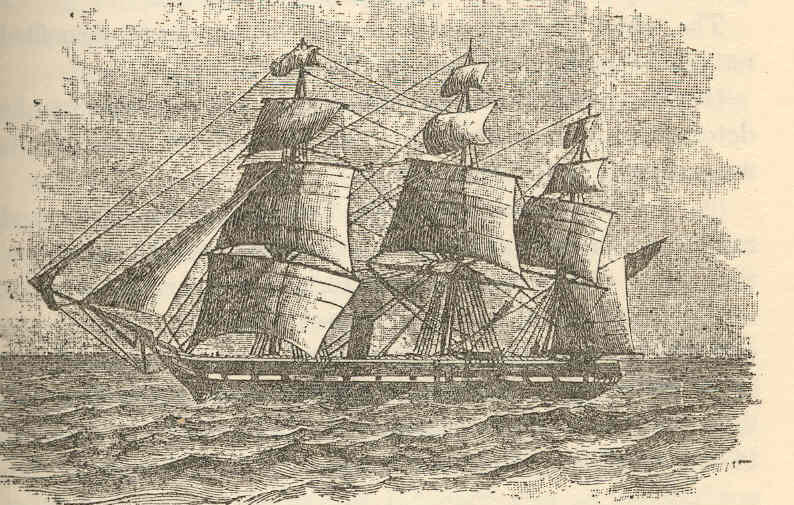
\includegraphics[width=0.55\linewidth]{images/book1/g8-challenger-sounding.jpg}

{\small HMS \emph{Challenger} preparing to sound the depth of the \omterm{def:g2:water-on-earth:ocean}{ocean},
1872. Engraving from the reports of the expedition, reproduced in
W.~A.~Herdman, \emph{Founders of Oceanography} (1923); public domain, via
Wikimedia Commons.}
% ledger: commons:challenger
\label{fig:g8:the-oceans:challenger}
\end{omfigure}

Today a ship \omterm{def:g2:drawing-to-map:map}{maps} the \omterm{def:g2:water-on-earth:ocean}{sea} floor with sound. A device under its hull sends
a short pulse of sound downwards; the sound bounces off the bottom and
comes back as an echo. The time the echo takes gives the depth, again and
again, while the ship keeps sailing. This is \emph{sonar}.
% ledger: nos:sonar

\begin{recall}
\omterm{def:g2:water-on-earth:salt-fresh}{Salt water} covers most of the Earth, in one world \omterm{def:g2:water-on-earth:ocean}{ocean} divided into
\omterm{def:g2:water-on-earth:ocean}{oceans} and \omterm{def:g2:water-on-earth:ocean}{seas} (\cref{ch:g2:water-on-earth}). \omterm{def:g7:plate-tectonics:plate}{Plates} move apart at the
\omterm{def:g8:the-oceans:seafloor}{ocean ridges} and one \omterm{def:g7:plate-tectonics:plate}{plate} sinks under another at the trenches
(\cref{ch:g7:plate-tectonics}). Over the \omterm{def:g2:water-on-earth:ocean}{oceans}, the winds blow in great
belts: \omterm{def:g8:winds-global-circulation:global-winds}{trade winds}, \omterm{def:g8:winds-global-circulation:global-winds}{westerlies} and \omterm{def:g8:winds-global-circulation:global-winds}{polar easterlies}, turned aside by the
Earth's rotation (\cref{ch:g8:winds-global-circulation}).
\end{recall}

\section{The ocean floor}

If the water of the \omterm{def:g2:water-on-earth:ocean}{oceans} could be drained away, a whole hidden
\omterm{def:g1:landscapes-around-us:landscape}{landscape} would appear. Along the \omterm{def:g1:landscapes-around-us:water}{coasts}, the land goes on under the \omterm{def:g2:water-on-earth:ocean}{sea}
as a gentle, shallow shelf. Then the floor plunges down a steep slope to
vast, flat \omterm{def:g1:landscapes-around-us:landform}{plains}, kilometres deep. \omterm{def:g4:world-physical-map:range}{Mountain ranges} rise from these
\omterm{def:g1:landscapes-around-us:landform}{plains}, and here and there narrow trenches go down deeper than anything
else on Earth.
% ledger: edin:challenger-stations

\begin{omfigure}
\begin{tikzpicture}[font=\footnotesize, >={Stealth[length=2mm]}]
  \fill[omSea] (0,0) rectangle (15.6,-4.2);
  \fill[omLithAlluv] (0,0.6) -- (1.2,0.15) -- (1.6,0) -- (3.4,-0.35)
    .. controls (3.9,-0.55) and (4.1,-2.6) .. (4.7,-3.1)
    -- (6.6,-3.35) -- (7.6,-3.1) -- (8.3,-2.2) -- (8.6,-1.7) -- (8.75,-1.9) -- (8.9,-1.65) -- (9.2,-2.3) -- (10.0,-3.15)
    -- (11.6,-3.4) -- (12.6,-3.45) -- (13.05,-4.1) -- (13.35,-3.0) -- (14.2,-0.9) -- (14.8,0.7) -- (15.6,1.3)
    -- (15.6,-4.6) -- (0,-4.6) -- cycle;
  \draw[black!70] (0,0.6) -- (1.2,0.15) -- (1.6,0) -- (3.4,-0.35)
    .. controls (3.9,-0.55) and (4.1,-2.6) .. (4.7,-3.1)
    -- (6.6,-3.35) -- (7.6,-3.1) -- (8.3,-2.2) -- (8.6,-1.7) -- (8.75,-1.9) -- (8.9,-1.65) -- (9.2,-2.3) -- (10.0,-3.15)
    -- (11.6,-3.4) -- (12.6,-3.45) -- (13.05,-4.1) -- (13.35,-3.0) -- (14.2,-0.9) -- (14.8,0.7) -- (15.6,1.3);
  \draw[omRiver] (1.55,0) -- (14.45,0);
  \node[anchor=south] at (8,0.05) {sea level};
  \node[align=center] at (2.6,-0.85) {continental\\shelf};
  \draw[->] (2.6,-0.55) -- (2.6,-0.25);
  \node[align=center, anchor=east] at (3.7,-2.0) {continental\\slope};
  \draw[->] (3.75,-2.0) -- (4.1,-1.9);
  \node[align=center] at (5.7,-2.6) {abyssal plain};
  \node[align=center] at (8.75,-0.9) {ocean ridge};
  \draw[->] (8.75,-1.15) -- (8.75,-1.55);
  \node[align=center] at (11.1,-2.6) {abyssal plain};
  \node[align=center, anchor=west] at (13.5,-3.9) {ocean\\trench};
  \draw[->] (13.45,-3.9) -- (13.15,-3.9);
  \node[anchor=south] at (0.8,0.6) {continent};
  \node[anchor=south east] at (14.7,1.0) {mountains};
\end{tikzpicture}

{\small The parts of the \omterm{def:g2:water-on-earth:ocean}{ocean} floor, from a \omterm{def:g1:landscapes-around-us:water}{coast} to the open \omterm{def:g2:water-on-earth:ocean}{ocean} and
another \omterm{def:g1:landscapes-around-us:water}{coast} (a sketch: depths and widths are not to scale).}
\label{fig:g8:the-oceans:sketch}
\end{omfigure}

\begin{definition}[The parts of the ocean floor]\label{def:g8:the-oceans:seafloor}
\begin{itemize}
  \item The \emph{continental shelf}\index{continental shelf} is the
        shallow, gently sloping edge of a \omterm{def:g3:continents-and-oceans:continent}{continent} under the \omterm{def:g2:water-on-earth:ocean}{sea}.
  \item The \emph{continental slope}\index{continental slope} is the
        steep slope that leads down from the shelf to the deep \omterm{def:g2:water-on-earth:ocean}{ocean} floor.
  \item An \emph{abyssal plain}\index{abyssal plain} is a vast, very flat
        and deep part of the \omterm{def:g2:water-on-earth:ocean}{ocean} floor.
  \item An \emph{ocean ridge}\index{ocean ridge} is a long chain of
        underwater \omterm{def:g1:landscapes-around-us:landform}{mountains} rising from the abyssal \omterm{def:g1:landscapes-around-us:landform}{plains}.
  \item An \emph{ocean trench}\index{ocean trench} is a long, narrow and
        very deep trough in the \omterm{def:g2:water-on-earth:ocean}{ocean} floor, often next to a chain of
        \omterm{def:g1:landscapes-around-us:landform}{mountains} or volcanic islands.
\end{itemize}
\end{definition}
% ledger: edin:challenger-stations, usgs:trench-depth

The \omterm{def:g2:water-on-earth:ocean}{ocean} is about \qty{3700}{m} deep on average, almost half the height
of the highest \omterm{def:g1:landscapes-around-us:landform}{mountain} on land. Its deepest point, the Challenger Deep in
the Mariana Trench in the Pacific \omterm{def:g2:water-on-earth:ocean}{Ocean}, is nearly \qty{11000}{m} below
the surface.
% ledger: nos:ocean-depth, usgs:trench-depth, tht:everest


\begin{method}[Reading a profile of the ocean floor]
\begin{enumerate}
  \item Read the axes: the distance across, the height or depth up and
        down, and the vertical exaggeration.
  \item Find \omterm{def:g4:world-physical-map:altitude}{sea level} (height 0) and the \omterm{def:g1:landscapes-around-us:water}{coasts} where the profile crosses
        it.
  \item Follow the floor from a \omterm{def:g1:landscapes-around-us:water}{coast}: the shallow shelf, the steep slope,
        then the deep flat \omterm{def:g1:landscapes-around-us:landform}{plains}.
  \item Look for what rises from the \omterm{def:g1:landscapes-around-us:landform}{plains} (a ridge) or drops below them
        (a trench), and read its depth.
\end{enumerate}
\end{method}

\begin{example}[Across the South Atlantic]
On the top profile, past the \omterm{def:g1:landscapes-around-us:water}{coast} of South America, the floor
drops to more than \qty{3000}{m} deep in less than \qty{300}{km}. \omterm{def:g8:the-oceans:seafloor}{Abyssal plains}, between
\qty{3500}{m} and \qty{5000}{m} deep, fill most of the width. Half-way
across, about \qty{4400}{km} along the profile, the Mid-Atlantic Ridge rises
to about \qty{2300}{m} below the surface: more than \qty{2000}{m} above
the \omterm{def:g1:landscapes-around-us:landform}{plains}, a \omterm{def:g4:world-physical-map:range}{mountain range} hidden under the \omterm{def:g2:water-on-earth:ocean}{sea}. The \omterm{def:g1:landscapes-around-us:landform}{plains} deepen again
to more than \qty{5000}{m} before the floor climbs to Africa.
\end{example}
% ledger: data:etopo1 (figdata/grade-8/seafloor_profile.py: ridge crest -2329 m at 4407 km; deepest -5295 m)

\begin{omfigure}
\begin{tikzpicture}
\begin{axis}[omsection, scale only axis, width=14cm, height=3.6cm, xmin=0, xmax=7569,
  ymin=-6000, ymax=1500, ytick={-6000,-4000,-2000,0}, xtick={0,1000,...,7000},
  xlabel={distance along 30.5\textdegree\ S, from 59.5\textdegree\ W (km)}, ylabel={height (m)},
  tick label style={font=\scriptsize}, label style={font=\small},
  yticklabel style={/pgf/number format/1000 sep={\,}}, xticklabel style={/pgf/number format/1000 sep={\,}},
  axis background/.style={fill=white}, clip=true]
  \fill[omSea] (axis cs:0,-6000) rectangle (axis cs:7569,0);
  \addplot[fill=omLithAlluv, draw=black!70, line width=0.5pt] table[x=km, y=elev_m] {figdata/out/grade-8-seafloor_profile-atlantic-rock.dat};
  \node[font=\scriptsize, align=center, fill=white, inner sep=1pt] at (axis cs:4407,-900) {Mid-Atlantic Ridge};
  \draw[-{Stealth[length=1.5mm]}] (axis cs:4407,-1250) -- (axis cs:4407,-2150);
  \node[font=\scriptsize] at (axis cs:2500,-5300) {abyssal plain};
  \node[font=\scriptsize] at (axis cs:6200,-5600) {abyssal plain};
  \node[font=\scriptsize, anchor=south west] at (axis cs:30,350) {South America};
  \node[font=\scriptsize, anchor=south east] at (axis cs:7380,350) {Africa};
  \node[anchor=north] at (rel axis cs:0.75,0.97) {\omve{260}};
\end{axis}
\end{tikzpicture}

\medskip
\begin{tikzpicture}
\begin{axis}[omsection, scale only axis, width=7cm, height=3.6cm, xmin=0, xmax=3020,
  ymin=-6000, ymax=4500, ytick={-6000,-4000,-2000,0,2000,4000}, xtick={0,1000,2000,3000},
  xlabel={distance along 20.5\textdegree\ S (km)}, ylabel={height (m)},
  tick label style={font=\scriptsize}, label style={font=\small},
  yticklabel style={/pgf/number format/1000 sep={\,}}, xticklabel style={/pgf/number format/1000 sep={\,}},
  axis background/.style={fill=white}, clip=true]
  \fill[omSea] (axis cs:0,-6000) rectangle (axis cs:3020,0);
  \addplot[fill=omLithAlluv, draw=black!70, line width=0.5pt] table[x=km, y=elev_m] {figdata/out/grade-8-seafloor_profile-pacific-rock.dat};
  \node[font=\scriptsize, align=center, fill=white, inner sep=1pt] at (axis cs:1300,1600) {Peru--Chile Trench};
  \draw[-{Stealth[length=1.5mm]}] (axis cs:1750,1150) -- (axis cs:1870,-5000);
  \node[font=\scriptsize, anchor=west] at (axis cs:2600,3500) {Andes};
  \node[font=\scriptsize] at (axis cs:700,-5300) {abyssal plain};
  \node[anchor=north west] at (rel axis cs:0.01,0.98) {\omve{148}};
\end{axis}
\end{tikzpicture}

{\small Two real profiles of the \omterm{def:g2:water-on-earth:ocean}{ocean} floor, from the ETOPO1 relief read
every degree of \omterm{def:g6:latitude-longitude:longitude}{longitude}. Top: across the South Atlantic, from South
America to Africa. Bottom: across the Pacific edge of South America. The
heights are stretched 260 and 148 times compared with the distances
(\emph{vertical exaggeration}), otherwise the \omterm{def:g2:water-on-earth:ocean}{ocean} would look as thin as
a sheet of paper; and with one point every degree, the narrow trench looks
shallower than it is.}
% ledger: data:etopo1, earth:Rmean (figdata/grade-8/seafloor_profile.py)
\label{fig:g8:the-oceans:profiles}
\end{omfigure}


\section{Salty water}

\omterm{def:g2:water-on-earth:ocean}{Sea} water tastes salty because salts are dissolved in it. Most of them
come from the \omterm{def:g3:stones-pebbles-sand:rock}{rocks} of the \omterm{def:g3:continents-and-oceans:continent}{continents}: \omterm{def:g4:clouds-rain-snow:precipitation}{rain} slowly wears the \omterm{def:g3:stones-pebbles-sand:rock}{rocks} away
and \omterm{def:g1:landscapes-around-us:water}{rivers} carry their dissolved salts to the \omterm{def:g2:water-on-earth:ocean}{sea}. Some come from hot
springs on the \omterm{def:g2:water-on-earth:ocean}{ocean} floor.
% ledger: nos:salinity-varies

\begin{definition}[Salinity]\label{def:g8:the-oceans:salinity}
The \emph{salinity}\index{salinity} of \omterm{def:g2:water-on-earth:ocean}{sea} water is the mass of salts
dissolved in a kilogram of \omterm{def:g2:water-on-earth:ocean}{sea} water. On average it is about
\qty{35}{g} per kilogram: \qty{3.5}{\%} of the mass of \omterm{def:g2:water-on-earth:ocean}{sea} water is
salt.
\end{definition}
% ledger: nos:salinity-varies

The \omterm{def:g8:the-oceans:salinity}{salinity} is not the same everywhere. When \omterm{def:g2:water-on-earth:ocean}{sea} water evaporates, the
water leaves but the salts stay behind: where the Sun is strong and \omterm{def:g4:clouds-rain-snow:precipitation}{rain}
is rare, the \omterm{def:g2:water-on-earth:ocean}{sea} becomes saltier. Where much \omterm{def:g4:clouds-rain-snow:precipitation}{rain} falls, or where a large
\omterm{def:g1:landscapes-around-us:water}{river} flows in, the \omterm{def:g2:water-on-earth:ocean}{sea} is less salty. When \omterm{def:g2:water-on-earth:ocean}{sea} water freezes into \omterm{def:g2:water-on-earth:ocean}{sea}
ice, the salt is left in the water around, which becomes saltier too.
On the whole, the \omterm{def:g8:the-oceans:salinity}{salinity} is low near the \omterm{def:g3:continents-and-oceans:equator}{equator}, where it \omterm{def:g4:clouds-rain-snow:precipitation}{rains} a lot,
and near the \omterm{def:g3:continents-and-oceans:poles}{poles}; it is highest in the middle \omterm{def:g6:latitude-longitude:latitude}{latitudes}, under the dry
belts near \ang{30}.
% ledger: nos:salinity-varies, nos:sea-ice-salt, mo:three-cells

\begin{omfigure}
\begin{tikzpicture}[font=\footnotesize, >={Stealth[length=2mm]}]
  \fill[omSea] (0,0) rectangle (13,-1.6);
  \draw[omRiver, line width=0.8pt] (0,0) -- (13,0);
  % left: dry belt, evaporation
  \fill[yellow!80!orange] (1.2,3.0) circle (0.35);
  \foreach \x in {1.0,1.8,2.6,3.4} \draw[->, black!50, line width=0.9pt, decorate, decoration={snake, amplitude=0.6mm, segment length=3mm}] (\x,0.15) -- (\x,1.6);
  \node[align=center] at (2.3,2.2) {strong evaporation,\\little rain};
  \node[align=center, fill=white, inner sep=1.5pt] at (2.3,-0.8) {\textbf{saltier}};
  % middle: rain
  \fill[black!20] (5.2,2.9) ellipse [x radius=1.3, y radius=0.4];
  \foreach \x in {4.4,4.8,...,6.0} \draw[omRiver] (\x,2.45) -- (\x-0.2,0.25);
  \node[align=center, fill=white, inner sep=1.5pt] at (5.2,-0.8) {\textbf{less salty}};
  \node at (5.2,3.55) {heavy rain};
  % right: river mouth and sea ice
  \fill[omLithAlluv] (7.4,0) -- (9.6,0) -- (9.6,0.6) -- (7.4,0.35) -- cycle;
  \draw[omRiver, line width=2pt, ->] (9.4,0.45) -- (7.9,0.2);
  \node[anchor=south] at (8.6,0.65) {river};
  \node[align=center, fill=white, inner sep=1.5pt] at (8.6,-0.8) {\textbf{less salty}};
  \fill[white, draw=omCold] (10.6,0.25) -- (12.6,0.25) -- (12.4,-0.25) -- (10.8,-0.25) -- cycle;
  \node[anchor=south] at (11.6,0.3) {sea ice forms};
  \node[align=center, fill=white, inner sep=1.5pt] at (11.6,-0.95) {\textbf{saltier}\\(salt left behind)};
\end{tikzpicture}

{\small What changes the \omterm{def:g8:the-oceans:salinity}{salinity} of the \omterm{def:g2:water-on-earth:ocean}{sea}: evaporation and freezing
leave the salts behind; \omterm{def:g4:clouds-rain-snow:precipitation}{rain} and \omterm{def:g1:landscapes-around-us:water}{rivers} add \omterm{def:g2:water-on-earth:salt-fresh}{fresh water}.}
% ledger: nos:salinity-varies, nos:sea-ice-salt
\label{fig:g8:the-oceans:salinity}
\end{omfigure}

\begin{omfigure}
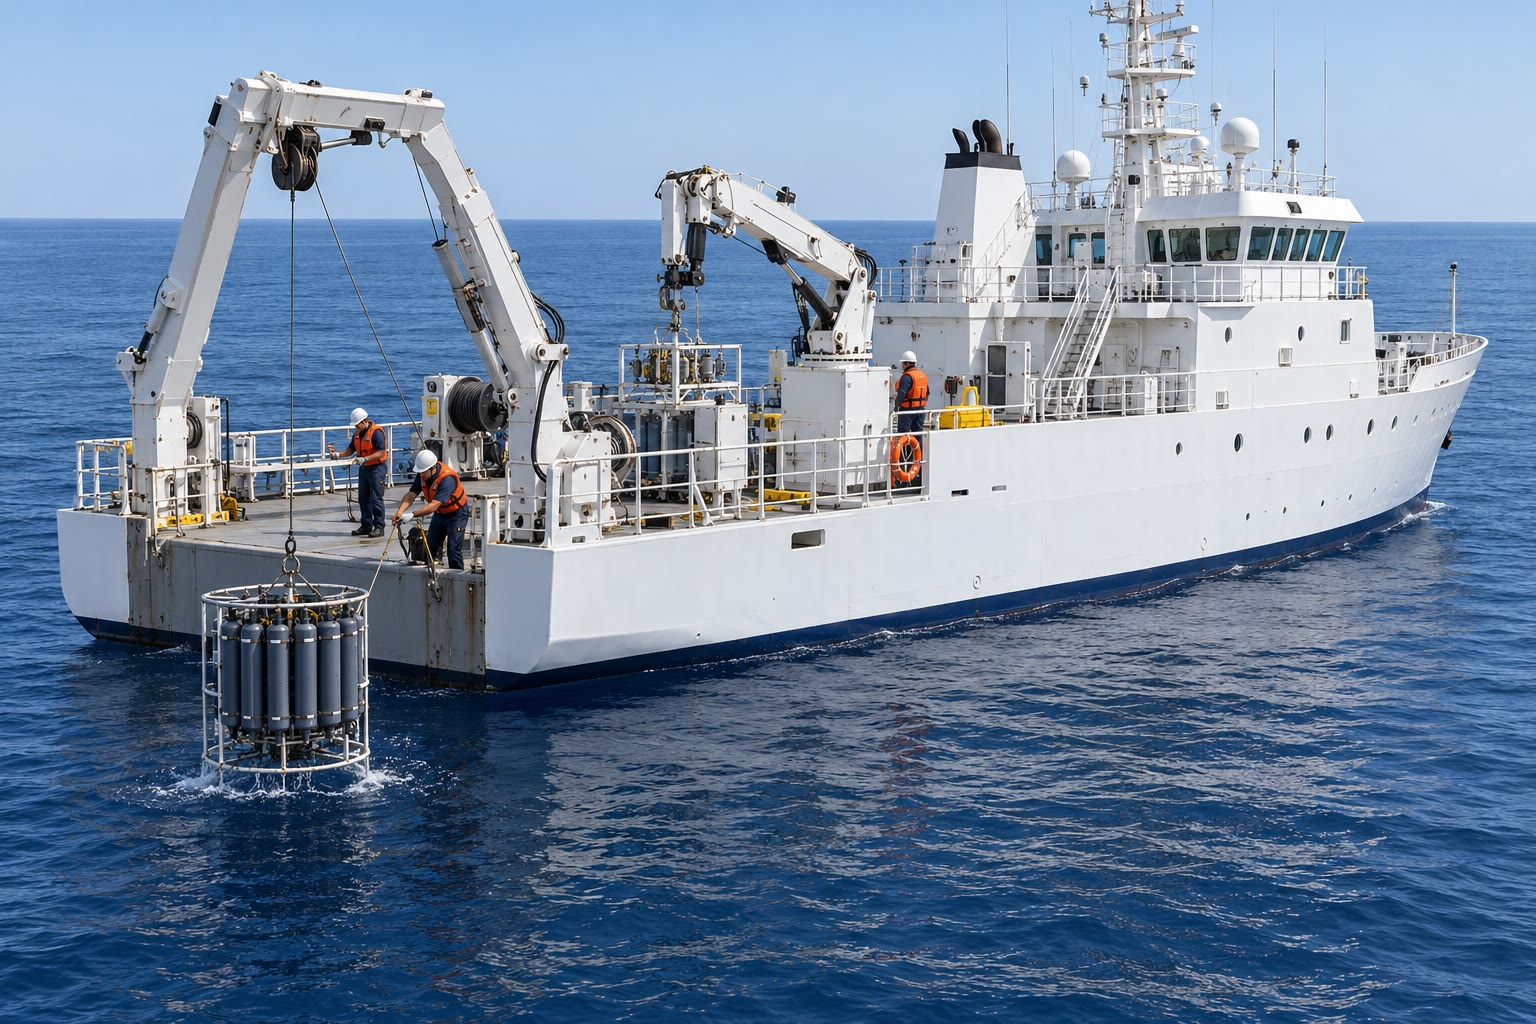
\includegraphics[width=0.58\linewidth]{images/book1/ai/g8-research-ship.jpg}

{\small A research ship lowers a frame of sampling bottles into the \omterm{def:g2:water-on-earth:ocean}{sea},
to bring back water from the depths and measure its saltiness and its
temperature (AI-generated illustration of a generic scene).}
\label{fig:g8:the-oceans:ship}
\end{omfigure}

\section{Currents at the surface}

The \omterm{def:g2:water-on-earth:ocean}{ocean} is never still. The winds drag on its surface and set the water
moving: the steady \omterm{def:g8:winds-global-circulation:global-winds}{trade winds} push it towards the west near the
\omterm{def:g3:continents-and-oceans:equator}{equator}, and the \omterm{def:g8:winds-global-circulation:global-winds}{westerlies} push it towards the east in the middle
\omterm{def:g6:latitude-longitude:latitude}{latitudes}. Like the winds, the moving water is turned aside by the
Earth's rotation: to the right in the \omterm{def:g3:continents-and-oceans:equator}{northern hemisphere}, to the left in
the \omterm{def:g3:continents-and-oceans:equator}{southern hemisphere}.
% ledger: nos:gyres

\begin{definition}[Ocean current and gyre]\label{def:g8:the-oceans:current}
An \emph{ocean current}\index{ocean current} is a steady movement of \omterm{def:g2:water-on-earth:ocean}{sea}
water in one direction, like a \omterm{def:g1:landscapes-around-us:water}{river} in the \omterm{def:g2:water-on-earth:ocean}{ocean}. A
\emph{gyre}\index{gyre} is a very large loop of \omterm{def:g2:water-on-earth:ocean}{ocean} currents that turns
round an \omterm{def:g2:water-on-earth:ocean}{ocean} basin.
\end{definition}
% ledger: nos:gyre-def, nos:gyres
\phantomsection\label{def:g8:the-oceans:gyre}

There are five great \omterm{def:g8:the-oceans:current}{gyres}: in the North and South Atlantic, in the North
and South Pacific, and in the Indian \omterm{def:g2:water-on-earth:ocean}{Ocean}. Those of the \omterm{def:g3:continents-and-oceans:equator}{northern
hemisphere} turn clockwise, those of the \omterm{def:g3:continents-and-oceans:equator}{southern hemisphere} anticlockwise.
On the western side of each \omterm{def:g2:water-on-earth:ocean}{ocean}, the \omterm{def:g8:the-oceans:current}{gyre}'s current is narrow and fast;
on the eastern side, it is broad and slow.
% ledger: nos:gyres

\begin{inthelab}[A gyre in a dish]
Indoors, fill a large round dish with water and sprinkle a pinch of pepper
on the surface. Blow gently and steadily across the dish through a straw,
always in the same direction, close to one edge. Watch the pepper: the
water near the surface starts to move with your breath, and soon the
whole surface turns in a loop round the dish.
\end{inthelab}

\begin{omfigure}
\begin{tikzpicture}
\begin{axis}[ommap, width=\linewidth, xmin=-180, xmax=180, ymin=-65, ymax=70,
  xtick={-180,-120,...,180}, ytick={-60,-30,0,30,60},
  xticklabels={$180^\circ$,$120^\circ$W,$60^\circ$W,$0^\circ$,$60^\circ$E,$120^\circ$E,$180^\circ$},
  yticklabels={$60^\circ$S,$30^\circ$S,$0^\circ$,$30^\circ$N,$60^\circ$N},
  tick label style={font=\scriptsize}]
  \addplot[fill=omLithAlluv, draw=black!45, line width=0.2pt] table {figdata/out/shared-geo-land.dat};
  \addplot[omWarm, line width=1.3pt] table {figdata/out/grade-8-ocean_currents-gyres-warm.dat};
  \addplot[omCold, line width=1.3pt] table {figdata/out/grade-8-ocean_currents-gyres-cold.dat};
  \addplot[quiver={u=\thisrow{u}, v=\thisrow{v}}, -{Stealth[length=2.6mm, width=2.2mm]}, omWarm, line width=1.3pt]
    table[x=lon, y=lat] {figdata/out/grade-8-ocean_currents-heads-warm.dat};
  \addplot[quiver={u=\thisrow{u}, v=\thisrow{v}}, -{Stealth[length=2.6mm, width=2.2mm]}, omCold, line width=1.3pt]
    table[x=lon, y=lat] {figdata/out/grade-8-ocean_currents-heads-cold.dat};
  \node[font=\scriptsize\bfseries, fill=white, inner sep=1pt, anchor=east] at (axis cs:-72,40) {Gulf Stream};
  \node[font=\scriptsize\bfseries, fill=white, inner sep=1pt, anchor=west] at (axis cs:-12,25) {Canary C.};
\end{axis}
\end{tikzpicture}

{\small The five great \omterm{def:g8:the-oceans:current}{gyres}, simplified: clockwise in the \omterm{def:g3:continents-and-oceans:equator}{northern
hemisphere}, anticlockwise in the southern. Red: warm currents, coming
from the \omterm{def:g5:weather-and-climate:tropics}{tropics}; blue: cold currents, coming from higher \omterm{def:g6:latitude-longitude:latitude}{latitudes}. The
North Atlantic \omterm{def:g8:the-oceans:current}{gyre} is edged by the Gulf Stream on the west and the Canary
Current on the east.}
% ledger: nos:gyres, data:ne-land (figdata/grade-8/ocean_currents.py)
\label{fig:g8:the-oceans:gyres}
\end{omfigure}

The best known of these currents is the Gulf Stream. It leaves the Gulf
of Mexico, runs north along the \omterm{def:g1:landscapes-around-us:water}{coast} of Florida, turns east off North
Carolina and crosses the Atlantic towards the north-east. Its warm water
moves on average at about \qty{6.4}{km} per hour, up to about \qty{9}{km}
per hour at the surface, and it carries more water than all the \omterm{def:g1:landscapes-around-us:water}{rivers} of
the world together. It keeps the east \omterm{def:g1:landscapes-around-us:water}{coast} of Florida warmer in winter
and brings mild air to western Europe.
% ledger: nos:gulf-stream, nos:gyres

\begin{omfigure}
\begin{minipage}[c]{0.5\linewidth}\centering
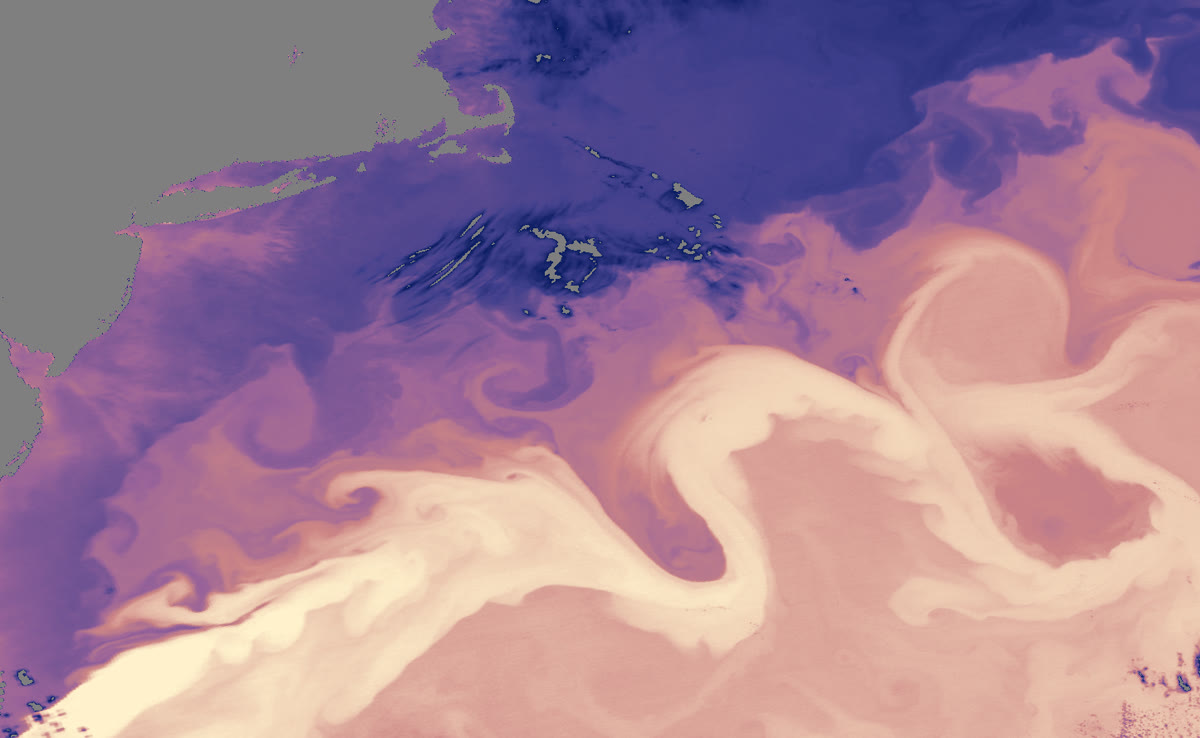
\includegraphics[width=\linewidth]{images/book1/g8-gulf-stream-sst.jpg}
\end{minipage}\hfill
\begin{minipage}[c]{0.46\linewidth}\raggedright
{\small The temperature of the \omterm{def:g2:water-on-earth:ocean}{sea} surface off the east \omterm{def:g1:landscapes-around-us:water}{coast} of North
America, measured by NASA's Aqua satellite on 18~April 2005. The Gulf
Stream is the band of warm water (light colours, up to about
\qty{23}{\degreeCelsius}) that winds from the bottom left towards the
right, between colder water (dark, down to about
\qty{-1}{\degreeCelsius}); land is grey. NASA (public domain, via
Wikimedia Commons).}
\end{minipage}
% ledger: commons:gulf-sst
\label{fig:g8:the-oceans:gulf}
\end{omfigure}


\section{Deep currents and the ocean's heat}

The winds drive the currents at the surface. Far below, in the cold
darkness of the deep \omterm{def:g2:water-on-earth:ocean}{ocean}, the water moves too, much more slowly. In the far North
Atlantic, the warm water brought by the Gulf Stream gives its heat to the
cold air; cooled, and made saltier when \omterm{def:g2:water-on-earth:ocean}{sea} ice forms, it becomes denser
and sinks to the bottom. This cold, salty water creeps south along the
\omterm{def:g2:water-on-earth:ocean}{ocean} floor, all the way to Antarctica, then into the Indian and Pacific
\omterm{def:g2:water-on-earth:ocean}{Oceans}, where it slowly rises and returns at the surface. A drop of water
can take about \num{1000} years to go once round this great loop, the
\emph{global \omterm{def:g2:water-on-earth:ocean}{ocean} conveyor belt}.
% ledger: nos:conveyor, nos:sea-ice-salt

\begin{omfigure}
\begin{tikzpicture}
\begin{axis}[ommap, width=\linewidth, xmin=-180, xmax=180, ymin=-65, ymax=70,
  xtick={-180,-120,...,180}, ytick={-60,-30,0,30,60},
  xticklabels={$180^\circ$,$120^\circ$W,$60^\circ$W,$0^\circ$,$60^\circ$E,$120^\circ$E,$180^\circ$},
  yticklabels={$60^\circ$S,$30^\circ$S,$0^\circ$,$30^\circ$N,$60^\circ$N},
  tick label style={font=\scriptsize}]
  \addplot[fill=omLithAlluv, draw=black!45, line width=0.2pt] table {figdata/out/shared-geo-land.dat};
  \addplot[omWarm, line width=1.3pt] table {figdata/out/grade-8-conveyor-surface.dat};
  \addplot[omCold, line width=1.3pt, dashed] table {figdata/out/grade-8-conveyor-deep.dat};
  \addplot[quiver={u=\thisrow{u}, v=\thisrow{v}}, -{Stealth[length=2.6mm, width=2.2mm]}, omWarm, line width=1.3pt]
    table[x=lon, y=lat] {figdata/out/grade-8-conveyor-heads-surface.dat};
  \addplot[quiver={u=\thisrow{u}, v=\thisrow{v}}, -{Stealth[length=2.6mm, width=2.2mm]}, omCold, line width=1.3pt]
    table[x=lon, y=lat] {figdata/out/grade-8-conveyor-heads-deep.dat};
  \node[font=\scriptsize\bfseries, fill=white, inner sep=1pt, anchor=west] at (axis cs:4,64) {sinks};
  \node[font=\scriptsize\bfseries, fill=white, inner sep=1pt, anchor=south] at (axis cs:163,11) {rises};
\end{axis}
\end{tikzpicture}

{\small The global \omterm{def:g2:water-on-earth:ocean}{ocean} conveyor belt, simplified to a single loop (a
sketch). Red: warm water at the surface; blue, dashed: cold, salty water
creeping along the deep \omterm{def:g2:water-on-earth:ocean}{ocean} floor. The water sinks in the far North
Atlantic, between Greenland and Norway, and rises in the Pacific (and,
not drawn, in the Indian \omterm{def:g2:water-on-earth:ocean}{Ocean}).}
% ledger: nos:conveyor, data:ne-land (figdata/grade-8/conveyor.py)
\end{omfigure}

\begin{example}[How slow is the deep water?]\label{ex:g8:the-oceans:deep-speed}
The loop drawn on the \omterm{def:g2:drawing-to-map:map}{map} is roughly \qty{70000}{km} long. If a drop of
water takes about \num{1000} years to go round it, it moves on average
about $\num{70000} \div \num{1000} = \qty{70}{km}$ a year, that is about
\qty{200}{m} a day. The Gulf Stream, at \qty{6.4}{km} an hour, covers about
\qty{150}{km} in a day: it goes as far in about 11 hours as the deep water
in a whole year.
% ledger: nos:conveyor, nos:gulf-stream, earth:Rmean (loop length and speeds computed in figdata/grade-8/conveyor.py)
\end{example}

Together, the surface and deep currents carry heat: warm water flows from
the \omterm{def:g5:weather-and-climate:tropics}{tropics} towards the \omterm{def:g3:continents-and-oceans:poles}{poles}, and cold water flows back towards the
\omterm{def:g3:continents-and-oceans:equator}{equator}. Like the winds, the \omterm{def:g2:water-on-earth:ocean}{ocean} evens out the uneven heating of the
Earth by the Sun.
% ledger: nos:conveyor, nos:gulf-stream, mo:global-circ

\section{Exercises}

\begin{exercise}[$\star$]\label{exo:g8:the-oceans:1}
Put these parts of the \omterm{def:g2:water-on-earth:ocean}{ocean} floor in the order in which a submarine meets
them as it leaves a \omterm{def:g1:landscapes-around-us:water}{coast} for the middle of the Atlantic: \omterm{def:g8:the-oceans:seafloor}{abyssal plain};
\omterm{def:g8:the-oceans:seafloor}{continental slope}; \omterm{def:g8:the-oceans:seafloor}{ocean ridge}; \omterm{def:g8:the-oceans:seafloor}{continental shelf}.
\end{exercise}

\begin{exercise}[$\star$]\label{exo:g8:the-oceans:2}
True or false? Correct the false sentences. (a) The \omterm{def:g2:water-on-earth:ocean}{ocean} is about
\qty{37}{km} deep on average. (b) The \omterm{def:g8:the-oceans:current}{gyres} of the \omterm{def:g3:continents-and-oceans:equator}{northern hemisphere}
turn clockwise. (c) Evaporation makes \omterm{def:g2:water-on-earth:ocean}{sea} water less salty. (d) The Gulf
Stream is a warm current.
\end{exercise}

\begin{exercise}[$\star$]\label{exo:g8:the-oceans:3}
Give the word for each description: (a) a long chain of \omterm{def:g1:landscapes-around-us:landform}{mountains} under
the \omterm{def:g2:water-on-earth:ocean}{sea}; (b) the mass of salt in a kilogram of \omterm{def:g2:water-on-earth:ocean}{sea} water; (c) a very large
loop of \omterm{def:g8:the-oceans:current}{ocean currents}; (d) a long, narrow and very deep trough in the
\omterm{def:g2:water-on-earth:ocean}{ocean} floor.
\end{exercise}

\begin{exercise}[$\star$]\label{exo:g8:the-oceans:4}
On the \omterm{def:g2:drawing-to-map:map}{map} of the \omterm{def:g8:the-oceans:current}{gyres}: (a) which way does the \omterm{def:g8:the-oceans:current}{gyre} of the South Atlantic
turn? (b) Name a warm current and a cold current of the North Atlantic.
(c) Which winds push the water towards the west near the \omterm{def:g3:continents-and-oceans:equator}{equator}?
\end{exercise}

\begin{exercise}[$\star\star$]\label{exo:g8:the-oceans:5}
A sample of \qty{1}{kg} of \omterm{def:g2:water-on-earth:ocean}{sea} water contains \qty{35}{g} of salts. (a)
What percentage of its mass is salt? (b) How many grams of salts are
there in \qty{20}{kg} of this water? (c) How many kilograms of \omterm{def:g2:water-on-earth:ocean}{sea} water
contain \qty{1}{kg} of salts?
\end{exercise}

\begin{exercise}[$\star\star$]\label{exo:g8:the-oceans:6}
A ship's sonar sends a pulse of sound straight down. The echo comes back
\qty{6}{s} later. Sound travels about \qty{1500}{m} each second in \omterm{def:g2:water-on-earth:ocean}{sea}
water. (a) How far does the sound travel in \qty{6}{s}? (b) Why is the
depth only half of this distance? (c) What is the depth? (d) Which part of
the \omterm{def:g2:water-on-earth:ocean}{ocean} floor could the ship be above?
\end{exercise}

\begin{exercise}[$\star\star$]\label{exo:g8:the-oceans:7}
Use the profile across the South Atlantic. (a) How deep are the \omterm{def:g8:the-oceans:seafloor}{abyssal
plains}, roughly? (b) At what distance along the profile is the crest of
the Mid-Atlantic Ridge, and how deep is it? (c) By how many metres does the
ridge rise above the \omterm{def:g1:landscapes-around-us:landform}{plains}? (d) Why does the profile need a vertical
exaggeration?
\end{exercise}

\begin{exercise}[$\star\star$]\label{exo:g8:the-oceans:8}
\omterm{def:g2:water-on-earth:ocean}{Sea} A lies between two \omterm{def:g5:weather-and-climate:desert}{deserts}: it hardly ever \omterm{def:g4:clouds-rain-snow:precipitation}{rains} there and no large
\omterm{def:g1:landscapes-around-us:water}{river} flows into it. \omterm{def:g2:water-on-earth:ocean}{Sea} B, in a rainy region, receives many large \omterm{def:g1:landscapes-around-us:water}{rivers}.
Explain which of the two is saltier than the open \omterm{def:g2:water-on-earth:ocean}{ocean}, and which is less
salty. Use the words \emph{evaporation}, \emph{\omterm{def:g2:water-on-earth:salt-fresh}{fresh water}}, \emph{salts
stay behind}.
\end{exercise}

\begin{exercise}[$\star\star$]\label{exo:g8:the-oceans:9}
A message in a bottle is thrown into the \omterm{def:g2:water-on-earth:ocean}{sea} off the \omterm{def:g1:landscapes-around-us:water}{coast} of Florida.
(a) Which current carries it first, and in which direction? (b) Which way
does it then cross the Atlantic? (c) If it went on round the \omterm{def:g8:the-oceans:current}{gyre}, along
which \omterm{def:g1:landscapes-around-us:water}{coast} would it travel south? (d) Is this current warm or cold?
\end{exercise}

\begin{exercise}[$\star\star$]\label{exo:g8:the-oceans:10}
The Gulf Stream moves on average at about \qty{6.4}{km} per hour. (a) How
far does its water travel in one day? (b) In a week? (c) Compare with a
person walking at \qty{5}{km} per hour.
\end{exercise}

\begin{exercise}[$\star\star\star$]\label{exo:g8:the-oceans:11}
The \omterm{def:g2:water-on-earth:ocean}{ocean} is about \qty{3700}{m} deep on average, and its deepest point is
nearly \qty{11000}{m} deep. (a) Write both depths in kilometres. (b) How
many times deeper than the average is the deepest point? Round to one
decimal. (c) A sonar echo from the deepest point: how many seconds does
it take to come back, at \qty{1500}{m} each second? (d) A drop of water
of the conveyor belt sinks in the North Atlantic. If it takes about
\num{1000} years to go round, how many years is that in powers of ten?
\end{exercise}

\begin{exercise}[$\star\star\star$]\label{exo:g8:the-oceans:12}
The great conveyor belt of the deep \omterm{def:g2:water-on-earth:ocean}{ocean} starts in the Norwegian \omterm{def:g2:water-on-earth:ocean}{Sea},
off the \omterm{def:g1:landscapes-around-us:water}{coast} of Norway, where warm water brought by the Gulf Stream gives
its heat to the cold air. (a) Using the \omterm{def:g8:the-oceans:current}{gyres} \omterm{def:g2:drawing-to-map:map}{map} and the chapter, explain
step by step how this warm water travelled there from the \omterm{def:g5:weather-and-climate:tropics}{tropics}, and
which winds pushed it. (b) Explain why the water then sinks. (c) Where
does it go next?
\end{exercise}

\section{Problem: A drifting buoy}

\begin{problem}[{Weekend problem --- a drifting buoy is launched off
Florida and carried round the North Atlantic gyre; its journey is followed
leg by leg, and the time it takes to go once round is worked out}]
\label{pb:g8:the-oceans:1}
% ledger: nos:drifter, nos:gulf-stream, nos:gyres (figdata/grade-8/ocean_currents.py; the leg lengths are rounded, the speeds of legs B to D are exercise data)
Scientists launch a drifting buoy off the \omterm{def:g1:landscapes-around-us:water}{coast} of Florida. It floats just
under the surface, moves with the currents, and sends its position to a
satellite. Its batteries last about one year. The \omterm{def:g2:drawing-to-map:map}{map} shows the four legs
of its journey round the North Atlantic \omterm{def:g8:the-oceans:current}{gyre}.

\begin{center}
\begin{tikzpicture}
\begin{axis}[ommap, width=11.5cm, xmin=-95, xmax=0, ymin=5, ymax=55,
  xtick={-90,-60,-30,0}, ytick={10,30,50},
  xticklabels={$90^\circ$W,$60^\circ$W,$30^\circ$W,$0^\circ$},
  yticklabels={$10^\circ$N,$30^\circ$N,$50^\circ$N},
  tick label style={font=\scriptsize}]
  \addplot[fill=omLithAlluv, draw=black!45, line width=0.2pt] table {figdata/out/shared-geo-land.dat};
  \addplot[black, line width=1pt, densely dashed, postaction={decorate, decoration={markings,
      mark=between positions 0.04 and 0.98 step 0.08 with {\arrow{Stealth[length=2mm]}}}}]
    table[x=lon, y=lat] {figdata/out/grade-8-ocean_currents-buoy.dat};
  \addplot[only marks, mark=*, mark size=2.2pt, omDef] coordinates {(-79.5,26)};
  \node[font=\scriptsize\bfseries, anchor=east, fill=white, inner sep=1pt] at (axis cs:-81,26) {launch};
  \addplot[only marks, mark=none, nodes near coords, point meta=explicit symbolic,
    every node near coord/.style={anchor=center, font=\footnotesize\bfseries, circle, fill=white, draw, inner sep=1pt}]
    table[x=lon, y=lat, meta=name] {figdata/out/grade-8-ocean_currents-buoy-legs.dat};
\end{axis}
\end{tikzpicture}

\medskip
{\small
\begin{tabular}{|c|l|c|c|}
\hline
leg & current & length (km) & average speed (km per day) \\
\hline
A & Gulf Stream & 3800 & 100 \\
B & North Atlantic Current & 2100 & 20 \\
C & Canary Current & 3100 & 20 \\
D & North Equatorial Current & 6100 & 20 \\
\hline
\end{tabular}}
\end{center}

\noindent\textbf{Part I --- The launch.}\par\nopagebreak
\begin{enumerate}[beginpenalty=10000]
  \item In which \omterm{def:g2:water-on-earth:ocean}{ocean}, and in which \omterm{def:g3:continents-and-oceans:equator}{hemisphere}, is the buoy launched?
  \item Which way does the \omterm{def:g8:the-oceans:current}{gyre} turn? Is the buoy carried north or south
        at first?
  \item Is the water of leg A warm or cold? And of leg C? Explain.
  \item Which winds drive the currents of leg B? Of leg D?
\end{enumerate}

\noindent\textbf{Part II --- Around the gyre.}\par\nopagebreak
\begin{enumerate}[resume, beginpenalty=10000]
  \item How many days does leg A take?
  \item How many days do legs B, C and D take?
  \item What is the total length of the journey round the \omterm{def:g8:the-oceans:current}{gyre}?
  \item Why is leg A so much faster than the others?
\end{enumerate}

\noindent\textbf{Part III --- The journey's length.}\par\nopagebreak
\begin{enumerate}[resume, beginpenalty=10000]
  \item How many days does the buoy need to go once round the \omterm{def:g8:the-oceans:current}{gyre}?
  \item Taking a month as 30 days, how many months is that? Round to the
        nearest whole month.
  \item On which leg will the batteries run out, after about one year
        (365 days)?
  \item How many more months of battery would the buoy need to send its
        position all the way round?
\end{enumerate}
\end{problem}
